% !TeX encoding = UTF-8
% !TeX spellcheck = en_US

% Document Version: v10

%*******************************************************************************
%* Work Configuration
%*******************************************************************************
\title{An Ontology of Student Consulting Organizations}
\author{Felix Förtsch}
\documentclass[a4paper, DIV=13, BCOR=0cm]{scrbook}

%*******************************************************************************
%* Packages
%*******************************************************************************
\usepackage[english]{babel}
\usepackage[urldate=iso]{biblatex}
\usepackage{xcolor} % Für Farben im Text
\usepackage{xstring} % String-Manipulation; wird von anderen Paketen oft verwendet
\usepackage{fontspec} % Einstellungen für Schriftarten (zB lokales Laden)
\usepackage{csquotes} % Verwaltet Anführungsstriche
\usepackage{hyperref} % Hyperlink-Helfer
\usepackage{paralist} % Erlaubt verschiedene neue Listen-Umgebungen (zB inparaenum)
\usepackage{mdframed} % Erlaubt das einfügen von Kästen (zB Einrahmen von Anmerkungen)
\usepackage{lscape} % Querformat-Umgebung
\usepackage[toc, section=section, numberedsection=autolabel]{glossaries} % Glossar
\usepackage[titletoc]{appendix}
\usepackage{progressbar}
\usepackage{tikz}

%*******************************************************************************
%* Configuration
%*******************************************************************************
% Language
\selectlanguage{english}

% Bibliography
\bibliography{main}
\KOMAoptions{bibliography=numbered}
\KOMAoptions{bibliography=leveldown}

% Table of Contents
%\setcounter{tocdepth}{\paragraphtocdepth}

% SubSubsection numbering
\setcounter{secnumdepth}{5}

% Layout Settings
\KOMAoptions{draft=false}
\KOMAoptions{twoside=false}
\KOMAoptions{titlepage=true}
%\KOMAoptions{headings=small}
\KOMAoptions{parskip=half} % Deaktiviert den den Absatzeinzug

% Header and Footer
\pagestyle{headings}
\KOMAoptions{headsepline=true} % Aktiviert eine Trennlinie zwischen Header und Dokument
%\KOMAoptions{footnotes=multiple}

% Style
%\setmainfont[
%	Path=Fonts/,
%	Extension=.ttf,
%	UprightFont=*,
%	BoldFont=*-Bold,
%	ItalicFont=*-Italic,
%	BoldItalicFont=*-BoldItalic
%]{DejaVuSerif}
%\setmonofont[
%	Path=Fonts/,
%	Extension=.otf,
%	UprightFont=*-Regular,
%	BoldFont=*-Bold,
%]{FiraCode}

%*******************************************************************************
%* Macros
%*******************************************************************************
\newcommand{\eg}{e.\,g.\ }
\newcommand{\Eg}{E.\,g.\ }
\newcommand{\aka}{a.\,k.\,a.\ }
\newcommand{\class}[1]{\texttt{\textbf{#1}}}
\newcommand{\relation}[1]{\texttt{#1}}
\newcommand{\prop}[1]{\texttt{#1}}
\newcommand{\pn}[1]{\textit{\textbf{#1}}}
\newcommand{\foottt}[1]{\footnote{\texttt{#1}}}
\newcommand{\link}[2]{\href{#1}{$\hookrightarrow$#2}}

%*******************************************************************************
%* Glossar
%*******************************************************************************
\glsdisablehyper % Disables hyperlinks for the glossary
\makenoidxglossaries

% Acronyms
\newacronym{sco}{SCO}{Student Consulting Organization}
\newacronym{je}{JE}{Junior Enterprise}
\newacronym{bdsu}{BDSU}{Bundesverband Deutscher Studentischer Unternehmensberatungen}
\newacronym{jcn}{JCNetwork}{Junior Consultant Network}
\newacronym{hc}{HC}{Hanseatic Consulting}
\newacronym{ci}{CI}{Campus Inform}
\newacronym{kiss}{KISS}{Keep It Stupid Simple}
\newacronym{aktg}{AktG}{Aktiengesetz}
\newacronym{gmbhg}{GmbHG}{Gesetz betreffend die Gesellschaften mit beschränkter Haftung}
\newacronym{foaf}{FOAF}{Friend of a Friend}
\newacronym{dcmi}{DCMI}{Dublin Core Metadata Initiative}
\newacronym{dcmt}{DCMT}{Dublin Core Metadata Terms}
\newacronym{bfo}{BFO}{Basic Formal Ontology}
\newacronym{gfo}{GFO}{General Formal Ontology}
\newacronym{fibo}{FIBO}{Financial Industry Business Ontology}
\newacronym{gist}{GIST}{GIST}
\newacronym{schema}{Schema}{Schema.org Ontology}
\newacronym{doap}{DOAP}{Description of a Project}
\newacronym{bpmn}{BPMN}{Business Process Modeling and Notation}
\newacronym{epc}{EPC}{Event-Driven Process Chain}
\newacronym{uml}{UML}{Unified Modeling Language}
\newacronym{psl}{PSL}{Process Specification Language}
\newacronym{nist}{NIST}{National Institute of Standards and Technology}
\newacronym{opm}{OPM}{Object Process Methodology}
\newacronym{hrp}{HRP}{Human Resource Process}
\newacronym{pp}{PP}{Project Process}
\newacronym{oc}{OC}{Organizational Context}
\newacronym{pc}{PC}{Project Context}
\newacronym{co}{CO}{Coporate Officer}
\newacronym{ceo}{CEO}{Chief Executive Officer}
\newacronym{cfo}{CFO}{Chief Financial Officer}
\newacronym{cto}{CTO}{Chief Technical Officer}
\newacronym{clo}{CLO}{Chief Legal Officer}
\newacronym{coo}{COO}{Chief Operating Officer}
\newacronym{iso}{ISO}{International Organization for Standardization}
\newacronym{pm}{PM}{Project Management}
\newacronym{owl}{OWL}{Web Ontology Language}
\newacronym{w3c}{W3C}{World Wide Web Consortium}
\newacronym{rdf}{RDF}{Resource Description Framework}
\newacronym{rdfs}{RDFS}{Resource Description Framework Schema}
\newacronym{skos}{SKOS}{Simple Knowledge Organization System}


%*******************************************************************************
%* Dokumentenanfang
%*******************************************************************************
\begin{document}

\titlehead{Overall Progress: \progressbar[filledcolor=yellow]{0.3}}
\subject{Bachelor's Thesis}
\title{Student Consulting Organizations}
\subtitle{A Domain Ontology}
\author{Felix Förtsch \\ 3708438}
\date{01.04.2020}
\publishers{Leipzig University}
\maketitle

\frontmatter
\chapter*{Abstract \progressbar[filledcolor=green]{1}}
	This work develops a domain ontology for \glspl{sco}. The model declares the domain knowledge and defines its vocabulary. It contains the information necessary to establish or run such an organization in a university context. Additionally it allows for optimization in existing organizations and contributes to cooperation between \glspl{sco} by organizing the existing knowledge. It maximizes the use of vocabularies, relations, and classes from established ontologies like \gls{foaf}, \gls{fibo}, \gls{gfo}, and \gls{gist} to link the domain knowledge into a bigger context. The main resource of the developed ontology are \glspl{sco} from Germany, but the concepts can be transferred and made applicable in a wider area.

\chapter*{Formatting}
\begin{compactitem}
	\item Hyperlinks are embedded and clickable in the PDF. They are marked with an arrow and a light blue border: \link{https://hyperlink.com}{Hyperlink}
	\item Everything related to the ontology implementation, such as references to classes or relations, is written as \texttt{typewriter text}.
	\item Relations are written in camelCase: \texttt{subclassOf}
	\item Classes are bold, capitalized, and use Snake\_Case: \texttt{\textbf{Awesome\_Class}}
	\item Name spaces may be added to a class for clarification; they are separated by a colon: \class{namespace:Class}
\end{compactitem}

% To raise awareness for unfairness in society, we use the female form of words where it is possible.

% TODO: Decide on labeling system \url{https://en.wikipedia.org/wiki/Simple_Knowledge_Organization_System}

\chapter*{Leseanleitung}
\newpage

\tableofcontents
\newpage

\mainmatter
\chapter{Introduction \progressbar[filledcolor=yellow]{0.6}}
\section{Motivation \progressbar[filledcolor=green]{0.8}}
\gls{sco}\footnote{Also known as \link{https://en.wikipedia.org/wiki/Junior_enterprise}{\glspl{je}} in some parts of the world.} are student-run consulting businesses, that focus on teaching their members essentials business and life skills exceeding the theoretical knowledge from university. They are very similar to small to medium consulting businesses, but are run and organized---most of the time exclusively---by students. And even though the concept is not universally know, these kind of organizations exists worldwide and have a history dating back to at least 1967\footnote{The founding of \link{https://www.en.junioressec.com/}{Junior ESSEC} in France.}. Germany has two different umbrella organizations for \glspl{sco} with more than 60 member organizations.\footnote{\link{https://bdsu.de}{\gls{bdsu}}, \link{https://jcnetwork.de}{\gls{jcn}}}

But as far as we know, there hasn't yet been any effort to collect and compose the existing domain knowledge of German \glspl{sco} in a publicly available and usable form. We consider this an important task, since it is a contribution to prevent knowledge loss that is inherent in the dynamics of these organizations: the majority of the staff are students and thus their consulting career is inherently linked to their university career:

\begin{enumerate}
	\item The career is time-bound to the duration of the education. A bachelor's degree in Germany averages 7,5-7,6 semesters and a master's degree 4,2-4,5 semesters, which adds up to a total of 11,7-12,1 semesters or ca. six years. \cite{stabu2019a} This frames the available time for the transfer of the domain knowledge.\footnote{There sometimes are also PhD students, but they can be considered outliers and are atypical.}
	\item The career is in parallel to the curriculum. From our experience, freshmen that decide to join student organizations typically do so at the beginning of their second or third semester, after they got acclimated with the workload of their university classes. Since students usually participate in parallel to their education---and the focus is typically on the education---, they have to manage their time accordingly, which reduce time spent with the \gls{sco}. Furthermore, students may have other (\eg personal) interests that compete with the same time budget.
\end{enumerate}

The reasons above reduce the available time for knowledge transfer and persistence and make these problems harder. Many \glspl{sco} have worked on and developed solutions to help with this problem. Some of them are informal, some formal in nature. For example: One particular organization, \link{https://hanseaticconsulting.de}{\gls{hc}}, used process methodology to document a lot of their knowledge.

However, the majority of available domain documents are highly individualized and miss the necessary level of abstraction to make them directly applicable to other \glspl{sco}. But even though every \gls{sco} is organized slightly differently than the next, uses different vocabulary and each has their individual culture, they all share the idea of teaching consulting and project work to their members. Since they aim for the same goal, they are very similar at their core.

Therefore we try to contribute a more general model in the form of an ontology that tries to combine the domain knowledge, vocabulary, and common concepts.

\section{Goal and Scope of the Work \progressbar[filledcolor=green]{1}}
\label{goal}
The goal of this work is the description of an abstract \gls{sco}. It extracts the available implicit expert knowledge, links it with related work, and transforms it into explicit  knowledge by using an ontology as its vehicle. It defines common classes and relations required to describe such an organization using domain vocabulary. Additionally it provides terminology explanations, background knowledge, and links into other ontologies where it is sensible.

\section{Deliverables \progressbar[filledcolor=green]{1}}
The output of this work are two documents:
\begin{enumerate}
	\item This thesis as a documentation and explanation of the ontology development process including but not limited to: methodology, background information, decisions in regards to the ontology, etc.
	\item The ontology document as a representation of the domain knowledge.
\end{enumerate}

\section{Out of Scope \progressbar[filledcolor=red]{0.1}}
\begin{compactenum}
	\item This work is not a thesaurus and not a documentation about a specific Student Consulting Organization.
	\item No diagram for individual orgs
	\item The ontology will not include the individual project process, since projects differ vastly between each other and more general ontologies and frameworks for projects already exists.
\end{compactenum}

\section{Outlook \progressbar[filledcolor=yellow]{0.5}}
The main motivation of this work is documenting the domain knowledge and making it available to interested parties, such as the umbrella organizations, \glspl{sco}, or students. Furthermore: Creating a computer-readable ontology with this goal in mind can help advance the idea of \glspl{sco}, for example by enabling software projects.

% TODO A formal ontology can be helpful in this task. \cite[p.\,252]{Jean_2007}

One particular use case in the intersection between knowledge management and software projects, is the creation of a tool that helps with founding new \glspl{sco} at universities where no \gls{sco} currently exists. Creating an organization without guidance is a daunting task; having a repository available, that structures and describes the elemental components of such an organization, can be a great help.

\chapter{Preliminaries \progressbar[filledcolor=yellow]{0.5}}
Ontologies have many applications in various fields. They are used in artificial intelligence research, database design and integration, semantic web, and many more. \cite[p.\,1]{Gomez-Perez:2004aa} One of these applications is knowledge representation.

\begin{quote}
	\enquote{Knowledge Representation is the field of Artificial Intelligence that focuses on the design of formalisms that are both epistemologically and computationally adequate for expressing knowledge about a particular domain.} \cite[p.\,XV, Preface]{baader2017introduction}
\end{quote}

This work is concerned with the knowledge representation of one particular domain: \glspl{sco}. The following section describes how we approach the development of this particular ontology, define the necessary vocabulary and relations between the terms, and structurally explore the domain.

\section{Methodology for the Development of the Ontology \progressbar[filledcolor=green]{0.95}}
% TODO: Minimal conceptual modeling opm principle (Model-based system engineering, page 77): minimal methodolgy is best

The primary goal of this work (see section \ref{goal})is the creation of a particular domain ontology. To achieve it, we start with the methodology that is proposed in the documentation \cite{guide-to-ontology} of the ontology editor \link{https://protege.stanford.edu}{\pn{Protégé}}---built and maintained by ontology researchers of \pn{Stanford University}. \cite{musen2015protege}

It involves the following steps:
\begin{compactenum}[(1)]
	\item Determine the domain and scope of the ontology,
	\item consider reusing existing ontologies,
	\item enumerate important terms in the ontology,
	\item define the classes and the class hierarchy,
	\item define the properties of classes-slots,
	\item define the facets of the slots, and
	\item create instances.
\end{compactenum}

It is important to note, that even though these steps look like they should be performed sequentially, this is not the case. Instead, the ontology starts out as a draft and is refined during development \cite[Section 3, Introduction]{guide-to-ontology}, following the iterative approach, that is common for ontology development. \cite[p.\,158, section 1.5.1]{stuckenschmidt2010ontologien} This quickly becomes apparent during the process of answering the suggested \pn{Competency Questions} to (1) determine the domain and scope of the ontology \cite[Section 3, Step 1]{guide-to-ontology} and taking into account (2) existing ontologies. And this also is true for steps (3) to (6). Therefore the steps are grouped together to make the overall structure of this work easier to follow.

The phases of the methodology are discussed in more detail in the following two sections and group the proposed steps as follows:

\begin{compactenum}
	\item Steps 1 and 2 are performed during the \pn{Research Phase}.
	\item Steps 3 to 6 during the \pn{Analysis and Synthesis Phase}.
\end{compactenum}

The last step, (7) the creation of instances, is omitted in this work. It is only really relevant if the ontology is used to describe one specific \gls{sco}. \cite{CN} However, this ontology is operating on a higher level of abstraction, trying to describe a more general case.

\subsection{Research Phase \progressbar[filledcolor=green]{1}}
To our understanding, the main goal of the first part of the methodology is the creation of a foundation for the ontology. It should have a clearly defined scope and its limits should be set. Additionally the recommended reuse of other ontologies helps creating a web of linked knowledge and reduces the amount of duplicate work.

To find a starting point for data collection and identify existing ontologies, we take an intuitive first look at \glspl{sco} and their driving factor:

\begin{mdframed}
	\textbf{The Idea of Student Consulting Organizations}\\
	Selecting a career is a very difficult and important choice in a young persons life. University education is closely linked to this choice and entering a specific field often requires a specific degree (\eg to become a lawyer, a student has to pass the bar exam).

	Most universities know this and have set up dedicated offices to offer career advice to their students. They not only help picking a fitting course of studies at the beginning of a university career, but also help the students to aim for a fitting job.

	Doing an internship with a company working in the field the student is interested in, is a widespread recommendation. It allows for a glimpse into the profession as well as gathering work experience.

	\glspl{sco} offer an option to investigate a career in business consulting, as well as learning the associated skills and getting paid in the process. They offer the students a way to learn about concept like project based work---the modus operandi of consulting companies---, \eg project planning and management, as well as structuring and presentation of information.

	Consulting is a very diverse field of work. Since consulting can be applied to any field of business, it can be used as a stepping stone into a career.
\end{mdframed}

Observing this intuitive perspective, we can see, that \glspl{sco} are connected to other knowledge domains in various ways: They are a type of social organization and thus are driven by people and processes. Organizations and in extension their processes have actors with responsibilities. This is a hint that the concept of roles might to be a part of the ontology. \glspl{sco} can be generally considered a form of business and therefore business aspects have to be taken into account. The fact that they do consulting work, creates a connection into the domain of (business) consulting and the domain of projects, since consulting work is project based.

This intuitive approach generates a the starting point for the research:
\begin{compactitem}
	\item Previously developed ontologies in related domains, \eg consulting, project management, educational organizations.
	\item Available domain knowledge, \eg process documentation of \gls{hc} and \gls{ci}.\footnote{Two \glspl{sco} the author has worked with the longest.}
	\item Personal expert domain knowledge and peer-review by other \gls{sco} members.
\end{compactitem}

Furthermore it implies some more general research topics:
\begin{compactitem}
	\item Implications of other general, upper-level, and top-level ontologies, \eg \gls{gfo}, \gls{bfo}, \gls{gist}.
	\item Theory of description logic and ontologies, \eg modeling of roles and processes.
\end{compactitem}

The results of this phase influence all parts of this work. However, some links are evident: The identified Related Work and the implications of higher-level ontologies as well as the classification can be found in section \ref{related-work}. The solutions to challenges of modeling the domain are discussed in sections \ref{general-aspects} and \ref{domain-aspects}.

Defining the scope of the ontology is the formal step that concludes the \textit{Research Phase}. This work accomplishes this by answering the Competency Questions. Since the questions can be considered a part of the ontology, they and their corresponding answers can be found as part of the ontology in section \ref{competency-questions}.

\subsection{Analysis and Synthesis Phase \progressbar[filledcolor=green]{1}}
\label{analysis}
The majority of this work happens during the Analysis and Synthesis Phase. Its goal is the review, interpretation, and structuring of the collected data; ultimately generating an ontology in the target format: \gls{owl}.

Based on the Protégé-methodology, the first two steps of this phase are: (3) the creation of an enumeration of terms that are relevant for the domain. And (4) the translation of the terms into the backbone of every ontology: the class hierarchy. Both are rooted in the results of the previous phase and further supplemented by expert knowledge.

At the core of this thought process is the conversion of available implicit knowledge into explicit knowledge. To help with it, we introduce a creative step: We start with a brainstorming to create a domain vocabulary collection in the form of a \textit{word cloud}. This simple first step involves writing down all the terms that might have something to do with the ontology. We then can transition this word cloud to a \textit{word graph}, by using the terms as vertices and implement associations between terms (\eg connected ideas or concepts) using the edges. We try to keep the word graph as simple as possible by focusing on the important connections and use existing vocabulary to prepare the links into other domains that will be done in the later stages of development.
% TODO: formally create word cloud

To progress from the word graph to the more rigorous class hierarchy, we transcribe the vertices into a first-draft/skeleton class hierarchy---using the Protégé editor---, starting with the most influential concepts. These can be identified by the amount of edges connecting them to other concepts; more connections indicate higher influence. Furthermore we can identify and assign trivial sub-classes during that process, by evaluating the quality of the edge connections. Fewer connections might indicate a more direct relationship between two terms. After these steps, the draft hierarchy contains mostly high-level classes and trivial sub-classes (\eg high-level class \textbf{Process} and all the identified processes as trivial sub-classes). It can then be further modified, refined, and polished by adding clarifications, delimitations, definitions, and descriptions to all terms as well as relations within the class hierarchy.

The output of final steps is the first major version of the ontology in the form of an \gls{owl} file, which completes the \textit{Analysis and Synthesis Phase} and also the second deliverable of this work. We document our most interesting observations during that process as part of this work.

\section{Definitions \progressbar[filledcolor=green]{1}}
Depending on the ambiguity and complexity of concepts, natural language can quickly become a limiting factor in terms of precision. Definitions are a tool to avoid confusion that arises from unclear semantics. To ensure a common understanding, this section discusses some key terms and their usage throughout this work.

\subsection{Vocabulary \progressbar[filledcolor=green]{1}}
Commonly, the term \textit{vocabulary} is used to describe the collection of all words one specific person knows. But this already implies that one person's vocabulary can be different to someone else's. Furthermore, the word vocabulary itself is also overloaded, as the dictionary definition (see appendix \ref{dictionary}) shows. Depending on context the described collection changes. \cite{mw-dictionary}

In the context of ontologies it is used interchangeably with \textit{alphabet} and \textit{signature}. On an abstract level it simply describes a set of symbols. \cite[p.\,46]{loebe2015ontological} Transferred to this work, it is the collection term for all class (see section \ref{classes}) and object property names (see section \ref{relations}), which are mainly words from the English language in conjunction with the underscore (\enquote{\_}) as delimitation symbol. The word choices draw inspiration or are translated from the \gls{hc} process documentation and our experience with different \glspl{sco}, as well as the business world. Some of these words are not special to the domain: \textbf{Organization}, for example, is not only used in many different related ontologies, but also very common in natural language.

To ensure adequate precision, each entry in the vocabulary has a few guaranteed properties (see section \ref{annotation-properties}).

\subsection{Domain Ontology \progressbar[filledcolor=green]{1}}
The term \textit{domain} is the easy part of this definition, since it intuitively and simply refers to the knowledge area it describes. \cite[p.\,7]{loebe2015ontological} This is close to the dictionary definition (see section \ref{dictionary}), where every listed sense has a delimiting meaning to it. \cite{mw-dictionary}

However, at the time of writing, an exact definition of the term \textit{ontology} is hard to come by. There is no unified understanding across the sciences. \cite{Hesse_2014} Numerous authors tried defining the term as shown by Loebe \cite[p.\,4-6]{loebe2015ontological} and Gomez et al. \cite[p.\, 6--9]{Gomez-Perez:2004aa}, but to our knowledge there has not yet been a conclusive definition. Since it's not our objective to end this discourse, we will not engage in a detailed analysis. Instead, we construct a \textit{working definition} by illuminating different aspects that are important for this work's goal of representing a knowledge domain.

The influential paper \cite[p.\,9]{schulz2012guideline} \cite[p.\,4]{loebe2015ontological} \textit{\enquote{A Translation Approach to Portable Ontology Specifications}} by Thomas R. Gruber---a paper that has been cited more than 19.000 times according to Google Scholar---contains the following definition:

\begin{quote}
	\enquote{An ontology is an explicit specification of a conceptualization.} \cite[p.\, 1]{gruber1993translation}
\end{quote}

Since it is on the more abstract sides for definitions, it is often used as a first step of narrowing down the intended meaning. Baader builds on it and proposes this slightly refined definition:

\begin{quote}
	\enquote{In computer science, an ontology is a conceptual model specified using some ontology language.} \cite[p.\,205]{baader2017introduction}
\end{quote}

This gives us two anchor points to attach it to our work:
\begin{inparaenum}
	\item Our ontology is a conceptual model of a \gls{sco}. We try to adhere as best as possible to the suggestions from the Good Ontology Guidelines: being formal, using explicit specifications, and being adequate for the domain it represents. \cite[p.\,10]{schulz2012guideline}
	\item Our ontology language of choice is \gls{owl}. It is an ontology language developed by the consensus-driven and well respected \gls{w3c}. \cite[p.\,206]{baader2017introduction} It is widely used and offers very good tooling in the ontology editor Protégé.
\end{inparaenum}

To works further towards our secondary goal of providing an ontology that is usable for software projects, we extend our requirements to the definition for domain ontologies from Jean: 

\begin{quote}
	\enquote{A domain ontology is a formal and consensual dictionary of categories and properties of entities of a domain and the relationships that hold among them.} \cite[p.\,240]{Jean_2007}
\end{quote}

We try to achieve formality by adhering to \gls{owl} standard and using the \textit{HermiT} reasoner during development. To aim for consensus, we prepare the ontology in way so that it can be peer reviewed in the future.

Similar to the general discussion about ontologies, there is an ongoing debate on which term best represents the elements of an ontology. We are following the Protégé naming convention and are calling the collection of elements \textit{entities}. Furthermore we use the term \textit{Classes} to represent things, \textit{Object Properties} to represent relationships between things, and \textit{Annotation Properties} to describe both more closely with additional comments.

\subsubsection{Classes and Class Hierarchy \progressbar[filledcolor=green]{1}}
\label{classes}
Classes are the most basic building blocks of an ontology. Each class tries to capture and describe an entity of the knowledge domain. The name of the class creates a connection between the entity within the ontology and the thing it tries to describe. It is supplemented by additional information via its annotation properties (see section \ref{annotation-properties}). The classes are aggregated an structured in a meaningful way by the \textit{class hierarchy}.

The class hierarchy is a tree where the children of a node have the built in relation (see section \ref{relations}): \relation{subclassOf}. There typically exists a root element called \class{Thing}, which \underline{all} classes are \relation{subclassOf}. As pointed out before, this work follows the \gls{owl} standard and hence we use \class{owl:Thing} as the root element; it has no properties. The built in relation gives additional meaning to classes in the hierarchy. \relation{subclassOf} implies that a class \relation{isA} type of the class it sub-classes. It is therefore key, to only introduce a sub-class relationship, if it is correct for the representation of the domain.

This has implications for our ontology. For example, it is the reason for the different structuring of \class{Agent} and \class{Process}: The former sub-domain can make use of the sub-class relation, whereas the latter cannot (see section \ref{process-subclass}).

\subsubsection{Properties \progressbar[filledcolor=green]{1}}
The classes and the class hierarchy give an ontology its basic structure; they defines what things exist in the world the ontology describes. The \textit{properties} bring this world to life. A property is a binary relation: It can be used to assert facts about a class, describe it in more detail, and to establish relationships between classes. \cite{w3c-owl-guide} We primarily use two types of properties in our work: \textit{Object Properties} and \textit{Annotation Properties}. To make them more distinguishable we also introduce and use their colloquial references \textit{Relationships}/\textit{Relations} and \textit{Annotations}.

\paragraph{Object Properties \aka Relationships \aka Relations}
\label{relations}
To express relationships within the knowledge area, we use object properties. The meaning of a thing is not only defined by its name and description, but also by the connections it has to other things. For example: A \class{Car} by itself invokes a certain image in the readers mind. Adding the relation \relation{hasBrandName} \class{Mercedes-Benz} changes the definition of the car by stipulating an additional restriction.

There are different ways of structuring object properties. The one end of the spectrum holds generalized relations, like \relation{hasA} or \relation{isPartOf}. This type of relationship can be applied to many different classes, because the semantics lies in the connection between the classes, instead of the relation itself. This type of generalized relation can be applied in different contexts. The \relation{isPartOf} relation, for example, can be used in different ways: A \class{Wheel} \relation{isPartOf} a \class{Car}; but also: A \class{House} \relation{isPartOf} a \class{Neighbourhood}.

On the other end fo the spectrum are highly specific relations that carry a lot of meaning by themselves and thus can not be applied to other contexts easily. For example: A \class{Person} \relation{isMemberOfTheMajorityCounil} \class{Member\_Council}.

As with many aspects of ontology development, it is important to strike the right balance and achieve the correct level of abstraction. In this work, we use a bottom-up approach. We start with specific relations and generalize them, if that is possible.

As already mentioned before, there is one special object property that is built into the class hierarchy: \relation{subclassOf}. It would be possible to It links a child class to its parent and expresses that the child is of the same type as the parent. For example: In our ontology, the class \class{Agent} is sub-classed by \class{Person} and \class{Organization}. This implies that both \class{Person} and \class{Organization} \underline{are} \class{Agents}. Everything a \class{Agent} can do, a \class{Person} or an \class{Organization} can also do.

\paragraph{Annotation Properties \aka Annotations}
\label{annotation-properties}
We use annotation properties to add additional information to entities in our domain. They can be thought of simple key-value pairs that are attached to a specific entity. The \underline{key} might be defined within the scope of the ontology or may be sourced from knowledge organization conventions like \gls{rdfs} or \gls{skos}. If a key belongs to such a schema, it uses the corresponding prefix, separated by a colon \enquote{:} (\eg \prop{rdfs:label}). The \underline{value} holds the additional information about a class.

Each class of our domain has two guaranteed annotation properties:
\begin{inparaenum}
\item A \prop{rdfs:label} to define its name in both English and German and
\item a \prop{rdfs:comment} in English, to describe the class more closely.
\end{inparaenum}
Furthermore we provide one or more \prop{skos:example} where examples help describing the class more clearly.

\section{Related Work and Classification}
\label{related-work}
As already discussed previously, the \gls{sco} domain touches on various other knowledge areas. Related source material could be found in other ontologies, \gls{pm} models and concepts, organizational theory, process documentation and models, established vocabulary, and so forth. The challenge lies in identifying the most useful information and merge the input from many different sources to construct the ontology.

This is made harder by the vastness of some related fields. \gls{pm}, for example, is a central topic for our domain and it is easy to find many different books, theories, and models about it on the market. It is also an complex, overarching, and very general subject matter. Part of its domain are concepts of complex nature like time, problem analysis, and project structuring. If we were to focus too much on this aspect within our ontology, it would easily dominate it and the ultimate goal of our ontology would be  missed. It is therefore imperative to identify the correct level of abstraction and connect the related work in an adequate manner.

This section discusses the related work and shows how we are applying it to the \gls{sco} ontology.



dcterms\footnote{\texttt{dcterms} is used in the \pn{FOAF} rdf file, \texttt{dct} is used in the \pn{FOAF} documentation.}


To reflect on this fact in the ontology, we try to merge the
\subsection{Top-Level Ontologies \progressbar[filledcolor=red]{0.1}}
\begin{compactenum}
	\item What is a TLO (Definition)?
	\item What can we use them for in this work? -> Processes, Roles, Time?
	\item What are popular TLOs and what are their strengths and weaknesses?
	\begin{compactenum}
		\item BFO %TODO: add note that BFO axioms are extensive and footnotes don't necessarily fully describe a class -> lookup needed
		\item DOLCE
		\item GIST
		\item BPMN  \cite{2014foisbpmn}
		\item GFO
	\end{compactenum}
\end{compactenum}

\subsection{Upper-Domain Ontologies}
\begin{compactenum}
	\item What is a UDO (Definition)?
	\item What can we use them for in this work?
	\item What are popular UDOs and what are their strengths and weaknesses?
	\begin{enumerate}
		\item OWL-S
		\item \href{https://en.wikipedia.org/wiki/Suggested_Upper_Merged_Ontology}{SUMO}
		\item \gls{fibo}
		\item \gls{doap} https://github.com/ewilderj/doap
		\item \gls{schema}: not really ideal, but useful for general concepts like Person or Organization
		\item \gls{foaf} is close to schema, link to dublin core: "dct:Agent
	\end{enumerate}
\end{compactenum}


Dublin Core's notion of Agent is much like FOAF's; Dublin Core says "A resource that acts or has the power to act.", we say "things that do stuff". As nobody has provided a counter-example of something fitting one definition but not the other, we say here that foaf:Agent stands in an 'equivalent class' relationship to dct:Agent (and vice-versa)." \cite[
External Vocabulary References]{Dan-Brickley2014FOAF-Vocabulary}



\section{Principles and Assumptions}
\label{general-aspects}

\subsection{Keeping Things Simple \progressbar[filledcolor=red]{0.2}}
\label{keeping-things-simple}
Polysemy Paper \cite{arapinis2015plea}
\gls{kiss}

keep it as simple as possible (\eg \textit{contract} and \textit{contract document} can be considered two distinct things, but this distinction is not important for the domain knowledge -- maybe add a relation "has document"?)

Example: A contract is a document that captures a business agreement. The word "contract" can refer to the immaterial agreement between the parties, but it can also refer to the document itself. Depending on the use case of the ontology it might be useful to separate these two things.

However, in this ontology the goal is to keep it a simple as possible, since the potential users of this ontology are not necessarily experts.

\subsection{The Open World Assumption}
\subsection{The Unique Name Assumption}
\subsection{Content Completeness Problem}
The \textit{Content Completeness Problem} states, that an ontology is incapable of containing all the concepts relevant to its users.

Developing an ontology involves thinking about the correct level of abstraction and making choices on what to focus on.

\url{https://en.wikipedia.org/wiki/Content_completeness_problem}
As is true for any domain ontology \cite{CN}, the content completeness problem exists for this ontology as well.

active/passive content completeness

bewusst weggelassen:
\subsubsection{Consulting Topics}
The main goal of consulting companies is in their name: consulting. They are a source of expertise and knowledge and can be employed as an option to solve a difficult problem at hand. The problem space of consulting companies is vast; examples are: Digitization, Human Resources, Knowledge Management, Market Research, Marketing, Coporate Strategy, etc. These topics are obviously part of the consulting domain. However, they are deliberately omitted, since their exploration would exceed the scope of the work.

\subsubsection{IT and Communication Systems}
IT systems are an essential part of modern business and there are companies where these systems are integral to everything (\eg AI companies). However, in the context of a consulting company they are mainly used to support, supplement, and optimize the already existing processes. Hence, a model of an IT system would not contribute in a meaningful way to the ontology.

\subsection{Time}
\label{time}
Implement time abstract -> only needed for processes before/after
no absolute time

\gls{bfo} \gls{gfo} have complex implementations of time that are not needed in this ontology.

\chapter{Ontological Aspects Specific to Student Consulting Organizations \progressbar[filledcolor=yellow]{0.4}}
\label{domain-aspects}
At the center of our domain lies a social structure. It is driven by processes and interactions that involve people. Such social constructs are inherently complex and dynamic. The same individual can often act in multiple capacities, aggregation of actors can occur in different degrees of formalization, the contexts of interactions are often fluid, etc.

In the following section, we discuss three major components of our ontology:
\begin{inparaenum}
	\item The different contexts that exist in the domain and how they influence other aspects of our model,
	\item human beings and how we organize them, and
	\item processes.
\end{inparaenum}

\section{Context and Context Switches \progressbar[filledcolor=red]{0.1}}
\begin{compactenum}
	\item Grundsätzliches Ziel von Ontologies -> Beschreibung von Wissen?
	\item Nutzung von natürlichsprachlichen Elementen -> Definition
	\item Diese Definition injeziert einen Context
	\item Begriffe bedeuten unterschiedliche Dinge je nach Kontext -> Kontext ist wichtig
	\item Allgemeiner Kontext in dieser Ontologie: genau 1 SCO -> Explizit andere SCO ausnehmen
	\item Referenz-Klasse: SCO
	\item Sub-Kontexte: PC/OC, etc
	\item Context Switching
\end{compactenum}

The goal of ontologies is the description of one particular knowledge area. Within it the ontology engineer defines

developed The context of an ontology defines

\label{context-switches}
We use the term \textit{context switching} in this work to describe the fact that some concepts influence instances of certain classes: They impose their context on the class. Even though individual instances are not in scope of this work, the implications of different contexts has to be taken into consideration while modeling the domain.

\subsection{Organizational Context}
\label{org-context}
The first context is the \gls{oc} and it is straight forward: The \gls{sco} itself is the primary and default context of the domain. It applies to all classes until otherwise stated. It is especially relevant for the internal formal structure of the organization. For example: It separates individuals that are involved with the \gls{sco} in any form from those that are not involved with it.

\subsection{Project Context}
\label{proj-context}
The second important context is the \gls{pc}. The central object and namesake of the context is the project. When reducing it to its most basic form, the project is an organizational construct that exists to reach a common goal.

\gls{iso} Definition: \enquote{A project is unique process, consisting of a set of coordinated and controlled activities with start and finish dates, undertaken to achieve an objective conforming to specific requirements, including the constraints of time, cost and resources} \cite{iso-9000-2015}



Another term connected to projects is project management

There exist a multitude of concepts, models, books, etc. on the topic.

It is a sub-context of the \gls{oc}, since projects are considered a part of the \gls{sco}

Each project on its own has its own context with associated roles

An \gls{sco} can be thought of as a central hub for multiple projects. It exists to generate the projects

\Eg a \class{Person} can be part of a project and part of the organizational structure at the same time.

\Eg a \class{Person}, can exist in different contexts at the same time.

The first two contexts are rooted in the nature of \glspl{sco}. On the one hand, they are organizations and as such have their internal structures, hierarchies, business ranks, etc. On the other hand they exists to provide project opportunities.

\subsection{Org-wide vs specific}

This pattern is not limited to a particular branch of the ontology.

\section{Social Constructs \progressbar[filledcolor=yellow]{0.7}}
 This section deals with the model for human beings.
 \eg as a \gls{sco} member or -non-member, as part of a project, as a customer, etc.
 Aggregation of these actors can occur in different degrees of formalization, \eg informal meeting of \gls{sco} members as friends, a project team meeting, an official meeting of the member council, etc. 

Since this is not a domain specific phenomenon, it is sensible to consider how existing and related ontologies (see section \ref{related-work}) represent these cases.

\subsection{General Implementation \progressbar[filledcolor=green]{1}}
\label{human-beings-in-other-ontologies}
Starting with the general model of human beings, \gls{foaf} is a very common choice when thinking about representing social structures. It is a well established ontology and referenced multiple times as backbone for social concepts. Its implementation and description are relatively basic: The anchor is the top-level class \class{foaf:Agent}\foottt{foaf:Agent rdfs:comment: \enquote{An agent (eg. person, group, software or physical artifact).}}, which is referred to as the class of \enquote{things that do stuff}. It is connected to the name space of the \gls{dcmt} via \relation{equivalentTo} \relation{dcterms:Agent}. It is sub-classed by
%
\class{foaf:Group}%
	\foottt{foaf:Group rdfs:comment: \enquote{A class of agents.}},
%
\class{foaf:Organization}%
	\foottt{foaof:Organization rdfs:comment: \enquote{An organization.}},
%
\class{foaf:Person}%
	\foottt{foaof:Person rdfs:comment: \enquote{A person.}},
%
\class{Person}%
	\footnote{\label{footn:no-desc}Note: The ontology doesn't offer any description.}, and
\class{schema:Person}%
	\footnote{See footnote \ref{footn:no-desc}.}.
\class{Person} and \class{schema:Person} are \relation{equivalentTo} \class{foaf:Person}.%
	\footnote{The link to \gls{schema} was added in the last update in 2014.} \class{foaf:Person} and \class{foaf:Organization} are disjoint. \class{foaf:Group} aggregates any type of \class{foaf:Agent}. \gls{doap} reuses exactly the same classes as \gls{foaf}. It also has the same links to \gls{schema} and \gls{dcmt}.

\gls{schema} implements
\class{schema:Person}%
	\foottt{schema:Person rdfs:comment \enquote{A person (alive, dead, undead, or fictional).}} and
%
\class{schema:Organization}%
	\foottt{schema:Organization rdfs:comment: \enquote{An organization such as a school, NGO, corporation, club, etc.}}.
%
\class{schema:Person} is considered \relation{equivalentTo} \class{foaf:Person}. This establishes a two-way link between \gls{foaf} and \gls{schema}. \class{schema:Organization} is sub-classed to accommodate for specialized forms of organizations that are relevant for the use cases schema was developed for, \eg \class{schema:Airline}, \class{schema:NGO}. A collection class like \class{foaf:Group} does not exists explicitly, but a \class{schema:Person} as well as a \class{schema:Organization} can be a \relation{memberOf} an \class{Organization}.

\gls{fibo} uses very similarly named classes with a more complex description. The root class is called
%
\class{fibo:AutonomousAgent}%
	\foottt{fibo-fnd-aap-agt:AutonomousAgent skos:definition: \enquote{An agent is an autonomous individual that can adapt to and interact with its environment.}}. It is sub-classed by
%
\class{fibo:Person}%
	\foottt{fibo-fnd-aap-ppl:Person skos:definition: \enquote{a person; any member of the species homo sapiens}}, %
%
representing individual humans. Like in \gls{foaf}, this class is disjoint with
%
\class{fibo:Organization}%
	\foottt{fibo-fnd-org-org:Organization skos:definition: \enquote{a unique framework of authority within which a person or persons act, or are designated to act, towards some purpose, such as to meet a need or pursue collective goals on a continuing basis}}.
%
\class{fibo:Group}%
	\foottt{fibo-fnd-org-fm:Group skos:definition: \enquote{a collection of autonomous entities}}
%
exists as a \relation{subclassOf}
%
\class{fibo:Collection}%
	\foottt{fibo-fnd-arr-arr:Collection skos:definition: \enquote{a grouping of some variable number of things (may be zero) that have some shared significance}}
%
and is described as collection of \class{fibo:AutonomousAgent}, which in turn is \relation{subclassOf}
%
\class{fibo:Arrangement}%
	\foottt{fibo-fnd-arr-arr:Arrangement skos:definition: \enquote{an organizing structure for something}}.
%
\gls{gist} offers the three classes
\class{gist:Person}%
	\foottt{gist:Person rdfs:comment: \enquote{NEGATIVE EXAMPLE: fictional characters.}},
%
\class{gist:Group}%
	\foottt{gist:Group rdfs:comment: \enquote{A collection of People. The group may or may not be an Organization. Many organizations consist of groups of people, but that is not a defining characteristic.}}, and
%
\class{gist:Organization}%
	\foottt{gist:Organization rdfs:comment:
		\begin{inparaenum}
			\item \enquote{A generic organization that can be formal or informal, legal or non-legal. It can have members, or not.},
			\item \enquote{EXAMPLES: Legal entities like companies; non-legal entities like clubs, committees, or departments.},
			\item \enquote{NOTE: There are a plethora of different kinds of organizations that differ along many facets, including members, structure, purpose, legal vs. non-legal, etc.}
		\end{inparaenum}
	}
as its implementation of the social structure.
However, the classes are organized very differently in the hierarchy and use the \relation{subclassOf} relation more extensively compared to \eg \gls{foaf}: To fully extract all information about the class \class{gist:Person}, its whole class path has to be taken into account.
A \class{gist:Person} is \relation{subclassOf}
%
\class{gist:LivingThing}%
	\foottt{gist:LivingThing rdfs:comment:
		\begin{inparaenum}
			\item \enquote{EXAMPLES: A cat, a mushroom, a tree.},
			\item \enquote{NEGATIVE EXAMPLES: fictional life forms such as Unicorns or Mickey Mouse.},
			\item \enquote{NOTE: In the open world, you must assume that it might have since died.},
			\item \enquote{Something that is now, or at some point in time was, alive and growing.}
		\end{inparaenum}
	},
which in turn is \relation{subclassOf}
%
\class{gist:PhysicalIdentifiableItem}%
	\foottt{gist:PhysicalIdentifiableItem rdfs:comment:
		\begin{inparaenum}
			\item \enquote{EXAMPLES: a computer, a book.},
			\item \enquote{NEGATIVE EXAMPLE:  A discontinuous thing like a manufacturing line cannot reasonably have an RFID attached to it, even though its parts are not the same kind of thing as the whole.},
			\item \enquote{NOTE:  You could, at least in principle, put an RFID tag on members of this class. Physical things are made of something.  E.g., statues are made of bronze.},
			\item \enquote{NOTE: In practice, this always means that the parts are not the same kind of thing as the whole.}
		\end{inparaenum}
	};
and both parent classes are carrying additional properties.
Similarly \class{gist:Group} is \relation{subclassOf}
%
\class{gist:Collection}%
	\foottt{gist:Group rdfs:comment:
	\begin{inparaenum}
		\item \enquote{Any identifiable grouping of instances.  For instance, a jury is a collection of people.},
		\item \enquote{EXAMPLES: A jury is a group of people,   a financial ledger is a collection of transaction entries; a route is an (ordered) collection of segments.}
	\end{inparaenum}}
with the limitation of every \class{gist:Group} \relation{hasMember some} \class{gist:Person}.

\gls{bfo} and \gls{gfo} don't offer any directly usable implementation for this specific problem, since they operate on a different level of abstraction.

When looking at the related work, we make the following observations:
\begin{enumerate}
	\item The modeling of human beings is concrete and intuitive: It operates on a low level of abstraction. Concepts that are in use by the layperson, \eg \class{Person} and \class{Organization}, are commonly used in reviewed ontologies; except for the top-level ontologies that operate on a much higher level of abstraction and are therefore not concerned with the concreteness of modeling human beings.
	\item The class \class{Agent} represents actors of an action. Sub-classing it gives the model freedom to express what exactly acts: It can be an \class{Agent}, a \class{Person}, a \class{Group}, or an \class{Organization}. This flexibility makes the models powerful. They can describe general (\eg somebody) or other agents (\eg robots) directly via \class{Agent}, but can also be used more specifically via a sub-class (\eg a \class{Person}). Additionally, a group is a collection class that is also \relation{subclassOf} \class{Agent} and hence can become an \class{Agent}---an actor---itself.
\end{enumerate}

As shown above, the classes \class{Agent}, \class{Person}, \class{Organization}, and \class{Group} are common in the class hierarchies of the related ontologies. Therefore this ontology will use these classes. However, the different ontologies also use different ways of defining classes. Ranging from the very direct and simple way of \gls{foaf}, to the very intricate way of \gls{gist}. Since this ontology is trying to be as intuitive to use as possible, the more simple approach from \gls{foaf} is adapted.\footnote{This decision is a direct application of the \gls{kiss} principle (see section \ref{keeping-things-simple}). Having more information in an ontology can obviously be useful for a very detailed model of a domain. However, its size can be kept smaller and the complexity lower by omitting information (\eg certain relations or attributes) that can be inferred from linked ontologies when necessary. For example: \gls{fibo} and \gls{gist} offer attributes for a \class{Person}; \eg in \gls{fibo} a \class{Person} \relation{hasDateOfBirth exactly 1} \class{Date}, in \gls{gist} a \class{Person} is \relation{offspringOf} another \class{Person} and need to have a \relation{name} \class{xsd:string}. These attributes can be extracted on demand, by following the \relation{equivalentTo} relation.}

After deciding on these basic building blocks, they can be extended according to the additional domain specifications. For example, a \class{Person} might need further differentiation based on \gls{sco} membership status, on business rank for internal organization and career progress, or on organizational roles. But there are other concepts that can involve a \class{Person}---\eg \enquote{\textit{being a customer} of the \gls{sco}}---that could just as easily involve an \class{Organization}. This observation points to the requirement of a more general approach for modeling these cases: Roles.

As already shown by \textit{Loebe}, the concepts and ideas about roles have been heavily discussed in the ontology community and literature. \cite[p.\,130~1.2]{loebe2007abstract} The role concept is not trivial, very fundamental, and using it as part of an ontology allows for a flexible and powerful model.
Since there is no clear agreement on a particular role concept, we are adopting the approach from \textit{Loebe} (2007) and its basic role model. It is very general and can be applied in various ways: It can be used in the intuitive way regarding social roles, \eg thinking about a human being playing the role of a patient and another the role of a doctor. But it is also possible to think about numbers and relationship between them in the form of abstract roles. \cite[p.\,131--133]{loebe2007abstract}

Since \glspl{sco} are a social construct and are defined by the people of the organization, the modeled roles are primarily from the type \textit{social role}. Furthermore, the contexts described in section \ref{context-switches} also have implications for the roles that exists in the domain.

\subsection{Roles in the Organizational Context \progressbar[filledcolor=green]{1}}

\subsubsection{Membership}
\label{membership}
Within the \gls{oc} (see section \ref{org-context}), the most basic property is membership: Either being part of the organization and thus being a \class{Member} or not participating and a \class{Non-Member}. \class{Members} of the \gls{sco} can play different roles in the \gls{oc}. \class{Non-Members} don't play roles within the organization, but can play external roles. For example: The role of a \class{Customer}. The distinction is important for this ontology, since the status is typically used in the internal organizational procedures. For example: Someone might be required to be a proper member to be allowed to vote in the Member Assembly, to be part of a project, or to become part of the Executive Board.

It is important to note, that within \glspl{sco} the \class{Member} role can only be played by human beings. For this model this means a restriction to \class{Person}. The members are the defining group that fills all the organizational functions, works on the projects, and participates in the majority of processes. Even though membership does not have to be limited like this in general---there are many examples where organizations are members of other organizations---it is limited in this domain. Since \class{Member} are necessarily \textbf{always} human beings, we introduce the role as \relation{subclassOf} \class{Person}.

The \class{Non-Member} role, however, is not limited to only \class{Person}. In fact, everything and everyone that is not a \class{Member} is by definition a \class{Non-Member}. Therefore it is sufficient to model the class \class{Member} and omit \class{Non-Member}.

\subsubsection{Business Ranks}
\label{ranks}
The second property a \class{Person} can have in the \gls{oc} is the business rank. Examples from the business world are: Associate, Senior Associate, Consultant, Partner, etc. Similar to regular businesses, \glspl{sco} also organize these ranks around their career process: A person receives the lowest available rank at the begin of their career. During the time with the organization a person is awarded higher ranks based on some organizational system (\eg a merit-based system), until the highest rank is reached or the person leaves the organization.

The exact terms for the ranks, their meaning, gradation, and organizational implications are highly specific to the \gls{sco} instance. We therefore introduce a rough and extensible skeleton representation:
\begin{compactenum}
	\item \class{Trainee}: The entry level rank, without a formal membership.
	\item \class{Junior Consultant}: The first rank after someone acquires an official, formal membership.
	\item \class{Consultant}: The rank that implies someone has reached the required amount of knowledge and experience to fulfill all organizational functions.
	\item \class{Senior Consultant}: The ultimate rank of the organization that can be reached after gathering a substantial amount of knowledge, experience, and organizational social status.
\end{compactenum}

\class{Ranks} can only be attained by \class{Members} and therefore both are directly related. Since a \class{Member} can only hold exactly one \class{Rank} and the \class{Rank} further specifies the \class{Member} in the \gls{oc}, we introduce the ranks as \relation{subclassOf} \class{Member}. This is similar to the \gls{schema} approach that sub-classes \class{Organization} to be more specific about the type of organization: We are sub-classing \class{Member} to be more specific about it.

\subsubsection{Corporate Officers}
The complete set of tasks and responsibilities for the organizations day-to-day leadership is associated with the group of people referred to as \glspl{co}. This set is typically divided into sub-sets and each sub-set is associated with a different role, to organize the work loads; and each role is played by a different person. For example: An organization may have the roles \gls{ceo}, \gls{coo}, and \gls{cfo} and each is played by a different individual.

The exact set of task differs from \gls{sco} to \gls{sco} and is also dependend on the organizational form, \eg a \gls{sco} using the form of a registered association has different (legal) obligations than a \gls{sco} organized as university group. Completely specifying it is impossible on the level of abstraction this ontology operates on. In the same vein, it is impossible to define which tasks are attributed to which role, since every \gls{sco} organizes differently. Therefore we fall back on an extensible model and introduce the general class \class{Coporoate\_Officer} as \relation{subclassOf} \class{Organizational\_Role}. To play a leadership role, it is required to be a formal \class{Member} of the \gls{sco}. Hence: \class{Coporoate\_Officer} \relation{isPlayedBy} only
(\class{Junior\_Consultant} or \class{Consultant} or \class{Senior\_Consultant}).

There exists some common roles, that arise from the necessities of an \gls{sco}: There is typically a person that is formally responsible for the organization, a person that takes care of the finances, and a person that takes care of legal aspects of the project work. We differentiate between these three branches explicitly and introduce dedicated roles for each: \class{Chief\_Executive\_Officer}, \class{Chief\_Financial\_Officer}, and \class{Chief\_Legal\_Officer}.

It is important to note that these roles can all be played by the $\underline{same}$ \class{Person}. And: That we do not introduce any concrete tasks these roles have to fulfill.

\subsubsection{Alumni, Advisor, and Patron}
In the duality of membership---\class{Member} vs. \class{Non-Member}---exists some roles, where an assignment to either group is not clear cut when projecting on the real world: Alumni, advisors and patrons. All of these roles can be played by \class{Members}, \class{Non-Members} or a \class{Group} of both. The role attribution depends on the internal organization of the particular \gls{sco}. Furthermore each of the roles have their own restrictions.

Alumni are a group of people that have been affiliated with an organization in the past, but are not members of that organization anymore. A good example are university alumni: The group of people that graduated from a specific university. Becoming an alumni typically is an informal and passive process that only requires previous \gls{sco} membership. However, it is also possible to interpret alumna as a more formal role and title, requiring being a \class{Member}. The common denominator in our model is the $\underline{previous}$ membership. Since this is a requirement and \class{Member} is restricted to be played by only \class{Person}, the same holds true for alumna. Furthermore, the previous membership also implies, that an alumna does not hold an internal rank anymore. We introduce \class{Alumna} as \relation{subclassOf} \class{Organizational\_Role}, restrict the player to \class{Person}, and specify a \relation{disjointWith} (\class{Trainee} or \class{Junior\_Consultant} or \class{Consultant} or \class{Senior\_Consultant}).

Advisors are selected (\eg appointed, chosen, elected) to assist the \gls{sco} leadership with a neutral perspective in their decisions. Becoming an advisor is an active, conscious process. Both parties, advisees and advisors, are necessarily restricted to \class{Person}: The leadership of the organization is recruited from the pool of members; and the advisory concept models a direct and personal exchange of assistance. We introduce \class{Advisor} as \relation{subclassOf} \class{Organizational\_Role} that can only be played by \class{Person}.

Patrons are financial and/or ideological supporters of the \gls{sco}: A financial patron directly contributes to the monetary funds of the organization; an ideological patron primarily supports the idea of \gls{sco} and contributes through non-financial means. Both roles can be played by one player simultaneously. Often times ideological patronage also involves a form of financial support and vice versa. For example: The associated university of the \gls{sco} may provide patronage (\eg allowing promotion on the university website and campus) and infrastructure (\eg offices, meeting rooms, etc.). We introduce \class{Patron} as \relation{subclassOf} \class{Organizational\_Role} and further specify \class{Financial\_Patron} and \class{Ideological\_Patron} as \relation{subclassOf} \class{Patron}. Since patronage, especially financial support, require contracts, the role can only be played by a formal entity: It is restricted to \class{Person} and \class{Organization}.

\begin{mdframed}
	\textbf{Note:} The model says nothing about social status and political power that typically come with ranks and roles, such as being a \gls{co} or advisor, within an organization (\eg a person that holds a rank or role for a long time may still have organizational power after stepping down: \link{https://en.wikipedia.org/wiki/Éminence_grise}{Éminence grise}).
\end{mdframed}

\subsection{Roles in the Project Context}
\subsubsection{Project Team: Member, Leader, Controller}
A project team in its most basic form consists of team members that are lead by a team leader. Additionally a project controller can be employed to observe and measure the progress of the project, giving feedback on the project work, and helping the team in various capacity where necessary. The controller role is usually played by a person that has gathered experience with projects and sharing them further supports the idea of \gls{sco} by furthering the learning process of the project team members.

We model the \class{Project\_Team} as \relation{subclassOf} \class{Group}, since it is a collection of people that play

We model \class{Project\_Team\_Member}

We model \class{Project\_Team\_Leader}

We model \class{Project\_Controller}

\subsubsection{Customer}
The second party of a project is the customer.

The \class{Customer} role can be played by an \class{Agent}


\subsection{Conclusion: Human Beings in this Work \progressbar[filledcolor=yellow]{0.4}}


The strength of the role concept is its flexibility. A player can play multiple roles at the same time and each role can be associated with a different context. An example for this is the CEO role. It has defined responsibilities and playing the role means a requirement to fulfill certain tasks. With \glspl{sco} typically any formal \class{Member}---in our ontology this means any \class{Member} with rank \class{Junior Consultant} or above---can become CEO by being elected. When elected, the \class{Member} plays two roles in the \gls{oc}. Additionally, the same \class{Member} could work on a project as \class{Project Leader}, a role from the \gls{pc}.



\section{Processes \progressbar[filledcolor=yellow]{0.4}}
Processes are a helpful concept when describing organizations: They are created to achieve a goal and its processes are the steps needed to reach that goal. \cite[p.\,5, Definition 1.1]{Weske:2019aa} In theory, every organization can be decomposed to a sequence of single activities, which, when executed correctly and in the correct order, terminate in reaching the goal of the organization.

Since processes are a commonly used concept in the business world, it is not surprising, that many different methods and frameworks for modeling them have been developed. Their output often are visual representations of all workflows that make up an organization. Combining process models with goals and measurements makes them a powerful tool for optimization and quality control. For example, ISO 9001 is an industry standard that uses a process approach as the foundation of measuring quality. \cite{iso-process-approach} Because process documentation contains a lot of data about organizations, it is a valuable source for ontology development.

Widely known representations and methods include: Flowcharts, \gls{bpmn}, \gls{epc}, \gls{uml} Activity Diagrams, and \gls{opm}\footnote{Standardized as ISO~19450.}. There are also contributions rooted in ontology research, such as the \gls{bpmn} ontology (an \gls{owl} ontology for the \gls{bpmn} notation) \cite{2014foisbpmn}, the \gls{psl}\footnote{Developed by the \gls{nist} and standardized as ISO~18629.}, and processes concepts as part of \gls{gfo} or \gls{bfo}.

\subsection{Implementation in Related Ontologies \progressbar[filledcolor=green]{0.5}}
% TODO: Was verfolgt die jeweilige Implementierung für ein Ziel? Irgendwie einen Schluss aus der betrachtung ziehen
When compared to the rather practical and direct implementation of social structures discussed in section \ref{human-beings-in-other-ontologies}, processes are a more abstract concept. The impact of abstraction levels clearly shows when analyzing related ontologies. For example: While \gls{foaf} is a good source when discussing its niche---the modeling of connection between human beings---it does not require an implementation of a process concept. The closest possible link between these two knowledge domains is the  class \class{foaf:Project}\foottt{foaf:Project rdfs:comment: \enquote{A project (a collective endeavour of some kind).}}, which can be viewed as a procedural concept. However, it doesn't offer any additional reusable detail.

A similar observation can be made for \gls{schema}. Its primary purpose is adding semantic meaning to the internet: \enquote{Schema.org is a collaborative, community activity with a mission to create, maintain, and promote schemas for structured data on the Internet, on web pages, in email messages, and beyond.} \cite{schema-mission} Hence, it is not surprising, that it doesn't implement a detailed process representation.

On the other hand, the two related top-level ontologies, \gls{bfo} and \gls{gfo}, deal with time (see section \ref{time}) on a very high level and also implement process concepts: \gls{bfo} uses the class
\class{bfo:Occurent}%
	\foottt{bfo:Occurent elucidation: \enquote{An occurrent is an entity that unfolds itself in time or it is the instantaneous boundary of such an entity (for example a beginning or an ending) or it is a temporal or spatiotemporal region which such an entity occupies\_temporal\_region or occupies\_spatiotemporal\_region. (axiom label in BFO2 Reference: [077-002])}}
%
as entry point for its process concepts. It is sub-classed by %
	\class{bfo:Process}\foottt{bfo:Process definition: \enquote{p is a process = Def. p is an occurrent that has temporal proper parts and for some time t, p s-depends\_on some material entity at t. (axiom label in BFO2 Reference: [083-003])}},
%
	\class{bfo:Process\_Boundary}\foottt{bfo:Process\_Boundary definition: \enquote{p is a process boundary =Def. p is a temporal part of a process and p has no proper temporal parts. (axiom label in BFO2 Reference: [084-001])}},
%
	\class{bfo:Spatiotemporal\_Region}\foottt{bfo:Spatiotemporal\_Region elucidation: \enquote{A spatiotemporal region is an occurrent entity that is part of spacetime. (axiom label in BFO2 Reference: [095-001])}}, and
%
	\class{bfo:Temporal\_Region}\foottt{bfo:Temporal\_Region elucidation: \enquote{A temporal region is an occurrent entity that is part of time as defined relative to some reference frame. (axiom label in BFO2 Reference: [100-001])}}.
%
Looking closer at the given examples\foottt{bfo:Process example of usage:
	\begin{inparaenum}
		\item a process of cell-division,
		\item a beating of the heart,
		\item a process of meiosis,
		\item a process of sleeping,
		\item the course of a disease,
		\item the flight of a bird,
		\item the life of an organism,
		\item your process of aging.
	\end{inparaenum}
} for \class{bfo:Process} emphasizes the classes high-level nature.

\gls{gfo} uses the class
\class{gfo:Processual\_Structure}\foottt{gfo:Processual\_Structure dc:description: \enquote{The category of processual structures centers around the more intuitive notion of processes. It captures processes themselves and occurrents, i.e., primarily structures of several other kinds that can be derived from processes.}}
as its entry point. It is sub-classed by
\class{gfo:Occurent}\foottt{gfo:Occurent dc:description: \enquote{The category of occurrents comprises several categories that can be derived from processes.}}
and
\class{gfo:Processes}\foottt{gfo:Processes dc:description: \enquote{Processes are directly in time, they develop over and unfold in time. Processes have characteristics which cannot be captured by a collection of time boundaries. In particular, processes exhibit internal coherence.}}.


\gls{doap}

\gls{fibo}

\gls{gist} uses the root class \class{Event}\foottt{gist:Event rdfs:comment: \enquote{Something happening over some period of time, often characterized as some kind of activity being carried out by some person, organization, or software application.}} to deal with time-related constructs such as processes.

bfp gfo contain valuable information, that can be modified and adapted for the process implementation of the \gls{sco} domain.


\subsection{Structure of the Class Hierarchy \progressbar[filledcolor=yellow]{0.6}}
\label{process-subclass}
Processes need special attention when implementing them in a domain ontology, since their nature is quite different from other classes that represent physical, \eg \class{Document}, or intuitive concepts, \eg \class{Person}. As mentioned in section \ref{classes}, the built in \relation{subclassOf} relation of the class hierarchy already carries semantic meaning, that is generally not applicable to processes. For example: a \class{Delivery\_Process} may involve a \class{Food\_Preperation\_Process} as a procedural step. However, it is easy to see and understand that a \class{Food\_Preperation\_Process} is $\underline{not}$ \relation{subclassOf} a \class{Delivery\_Process} and therefore should not inherit its properties.

To model processes correctly, one could consider introducing a class like \class{*\_Process\_Part} (in the given example: \class{Delivery\_Process\_Part}) and use it to collect and connect sub-processes to their parent process. However, this results in many additional \textit{helper} classes in the class hierarchy, since every level of sub-processes requires another \class{*\_Process\_Part} class. This makes the class hierarchy harder to read and understand, since the process structure is encoded in these helper classes.

Another solution is the use of a root \class{Process} class to collect all processes and the relation \relation{isProcessPartOf}\footnote{Inverse: \relation{hasProcessPart}.} to connect a sub-process to its parent process. This results in a completely flat structure of the class hierarchy: every process is directly \relation{subclassOf} \class{Process}, independent from the level of abstraction.

\subsection{Ordering of Processes \progressbar[filledcolor=red]{0.2}}
Another aspect that has to be discussed is the ordering of processes.

Processes are a concept that heavily relies on abstraction. The right level of abstraction depends on the use case.

\begin{compactenum}
	\item It is hard to create a complete process diagram/describe a complete process
	\item A successful process model relies on the correct
	\item Besides from the problem of completeness, if you go on the lowest level of abstraction ordering the steps become easier (true?!)
	\item Trying to create a generally applicable domain ontology brings up an interesting questions in regards to process concepts: what is the correct level of abstraction and is it possible to bring certain processes in the correct order
	\item It is therefore necessary to look at every process and its parts -- and discuss if 1) correct level of abstraction 2) can it be ordered
	\item A parent process aggregates child process

	\item When discussing the lowest level of a process Depending on the level of abstraction,
	\item Indepentendt from the class hierarchy problem, another topic: The procedural information is encoded in the relation.
	\item Processes are a sequence of action -> but not always
	\item there should be a next\_process relation, but it's not straight forward, since there is not necessarily a strict ordering.
	\item introduce a non strict ordering?
\end{compactenum}

\subsection{Discreet Events and Liquid Processes}

\begin{compactenum}
\item In addition to that a distinction has to be made between \textit{discreet} events and \textit{liquid} processes. \cite[p.\,447]{Russell:2010aa}
\item Processes are an immaterial concept that is strongly connected to relations of relative time, such as \relation{before} and \relation{after}.
\end{compactenum}




\subsection{Legal Requirements in the Processes \progressbar[filledcolor=red]{0.1}}
\glspl{sco} are organizations in the social context; German law applies to them, like it applies to every other German organization. It influences their structure and processes. However, discussing the impact of the law onto internal workings of an organizations would go far out of scope of this work. Therefore the ontology omits a detailed description of the legal obligations, but references them abstractly where it is necessary.

For example: German law requires every company to pay taxes on their earnings. Depending on the \gls{sco} and the way projects are handled, this influences the process that is concerned with taxation. To develop a perfectly correct model, a very detailed discussion of specific processes would be required; this is out of scope. However, interacting with the tax authorities and learning about and filing the correct paper work is an important part of the learning experience for student consultants. It is therefore important for the ontology. To address this fact, but keep the ontology focused, it is condensed into the class \textit{Project Taxation Process} as part of the \textit{Project Process}.


\subsection{Implementation of Processes in this Work \progressbar[filledcolor=red]{0.2}}
They intuitively have a start, duration, and end.

Since the focus of the ontology is on simplicity, we decide to use a single  class \class{Process} as root for all processes in conjunction with the \relation{isProcessPartOf} relation. This method utilizes the core concepts of ontologies, classes and relations, and avoids encoding extra information in unconventional ways. To compensate for the resulting un-intuitive flat class hierarchy, we add diagrams to describe the processes and their relationships graphically (see appendix \ref{process-diagrams}).

%\subsubsection{Intuitive Look}
The primary goal of an \gls{sco} is teaching students project work. They reach this goal by training their members and offering them opportunities to work on real-world projects. Looking at this from a high-level process perspective, this can be boiled down to distinct steps that have to be performed by the organization:

\begin{compactitem}
	\item Members have to be recruited.
	\item Members have to be taught the necessary skills, to be able to work on projects.
	\item Projects have to be acquired.
	\item Projects have to be worked on by members.
\end{compactitem}

Additionally these steps have various amount of support processes that help facilitate them, \eg technical and legal support.

%\subsubsection{Comparison with Process Documentation}
Conflating this intuitive view results in two complex processes that are commonly know in the business world \cite{CN} and are also present in the available process documentation \cite{HCPD}:
\begin{compactenum}
	\item A \gls{hrp}, that focuses on the recruitment, training, and generally enabling of human beings (or in the case of \glspl{sco}: Members).
	\item A \gls{pp}, that documents the way an organization handles projects from start to finish.
\end{compactenum}

Again, both processes are influenced by the context switches discussed in section \ref{context-switches}. On the one hand, they can be viewed as an individual instance for one of the main protagonists of the process. On the other, they can viewed as the process of the organization. Example:
\begin{compactitem}
	\item The main protagonist of the HRP is one individual student. This individual student is following one instance of the HRP; this instance does not have to be identical with the instance of a second individual student, nor with the planned process of the organization. Both individuals might do different educational courses, hold different business ranks within the organization, or might be at different points in time of their career.
	\item The \gls{sco} itself has a HRP. It structures important aspects of the organization such as the career path. It describes the complete path from recruitment of a new member to offboarding at the end of the membership. Most importantly this process describes the plan on an abstract level and knowingly omits parts of the real world process that are not important to the organization.
\end{compactitem}

\chapter{Student Consulting Organizations: The Ontology \progressbar[filledcolor=red]{0.2}}
\section{Scope of the Domain \progressbar[filledcolor=green]{0.8}}
\label{competency-questions}
\subsection{What is the domain that the ontology will cover? \progressbar[filledcolor=green]{1}}
\glspl{sco} are a form of consulting firms.  They can be compared to small consulting businesses, but are staffed -- most of the time exclusively -- by students. In other countries, \eg in France and Brazil, they are also referred to as \href{https://en.wikipedia.org/wiki/Junior_enterprise}{\textit{Junior Enterprises}} (JE). In Germany they are usually a registered association (German: \textit{Verein}) and/or a group associated with a specific university (German: \textit{Hochschulgruppe}). They aim to teach students about consulting as a profession by providing a platform that educates and trains students in the craft and provides them with the organizational means to work on consulting projects.

The domain is a specialization of the a classical consulting firm. It differs especially in terms of professionalization, since companies are focused on profit using education as the means, whereas \glspl{sco} focus on the educational aspect and on providing experience, while having profit as secondary goal.

\subsection{For what we are going to use the ontology? \progressbar[filledcolor=green]{0.8}}
This ontology is a contribution to the knowledge management of \glspl{sco}. It can be used to learn or teach about the domain. It can also be used as a starting point for projects that require a model of the domain.

\subsection{For what types of questions the information in the ontology should provide answers? \progressbar[filledcolor=green]{0.8}}
The ontology serves as an abstract description of the \gls{sco} domain. It defines all classes and relations that are typically present in this type of organization. Therefore it can answer questions like:
\begin{itemize}
	\item What processes exist and are required in an \gls{sco}?
	\item What roles exist and have to be filled in an \gls{sco}?
\end{itemize}

\subsection{Who will use and maintain the ontology? \progressbar[filledcolor=green]{1}}
The users of this ontology are the leadership of \glspl{sco} in Germany as well as the leadership of the \gls{sco} umbrella organizations. The release version coincides with the finalization and grading of this work. If the ontology sees use by the target group, it will be maintained by the author. Access will be publicly provided on a GitHub repository. It is considered a living document, hence not necessarily complete until otherwise stated. Contributions and forks will be possible via the GitHub interface.

\section{Classes}
\subsection{Agent}
\subsubsection{Group}
\subsubsection{Organization}
\subsubsection{Person}
\paragraph{Trainee}
\paragraph{Junior Consultant}
\paragraph{Consultant}
\paragraph{Senior Consultant}

\subsection{Document}

\subsection{Processes}

\subsubsection{Human Resource Process}
\subsubsection{Project Process}
\subsubsection{Support Processes}
\subsection{Projects}

\section{Relations}

Syntactic decision: is/has relations

% TODO: Verify ($\diamond$ means the relation is implemented in the ontology)

\textbf{Agent}
\begin{compactitem}
	\item All members except trainees and almunus can be corporate officers $\diamond$
	\item Non-members can't become corporate officers $\diamond$
	\item Members can play project team roles $\diamond$
	\item Every agent can play the customer role in a project $\diamond$
	\item Every member goes through his individual HRP
	\item An organizational rank has tbd requirements
	\item Customer, Team, Contract, etc are \textbf{part of} a project
	\item Organizations can only \textbf{play} the customer \textbf{role} in a project $\diamond$
	\item Organization can only play external roles $\diamond$
\end{compactitem}

\textbf{Processes}
\begin{compactitem}
	\item All processes have a \textbf{next\_process} $\diamond$
	\item \textbf{previous\_process} should be inferred?!
	\item
\end{compactitem}

before/after:
\begin{compactitem}
	\item FIBO: relates to -> precedes/succeeds?
	\item plays role
\end{compactitem}


\chapter{Conclusion}
\chapter{Further Research}

\appendix
\chapter{Appendix}
\section{Term Enumeration}
\label{word-cloud}

\newpage
\section{Diagrams}
\subsection{General Diagrams}
% TODO: Add correct relation

\begin{figure}[h]
	\caption{Ranks}
	\centering
	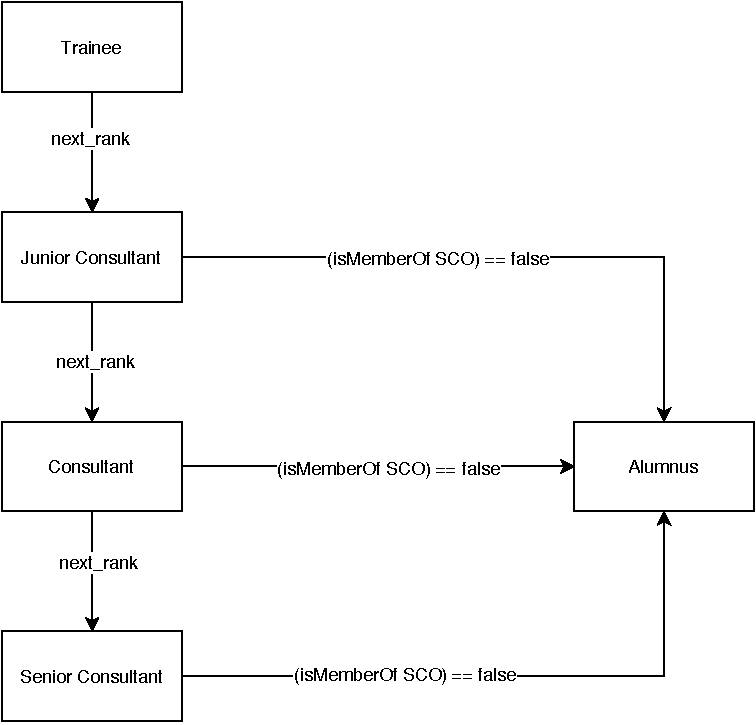
\includegraphics[width=1\textwidth]{Diagrams/ranks.pdf}
\end{figure}

\begin{figure}[h]
	\caption{Corporate Officers}
	\centering
	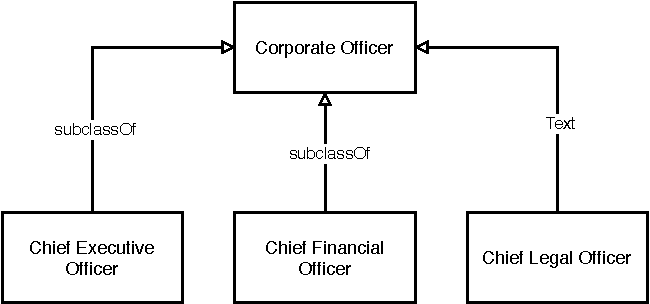
\includegraphics[width=1\textwidth]{Diagrams/corporate-officers.pdf}
\end{figure}


\clearpage
\subsection{Process Diagrams}
\label{process-diagrams}
\begin{figure}[h]
	\caption{Project Process}
	\centering
	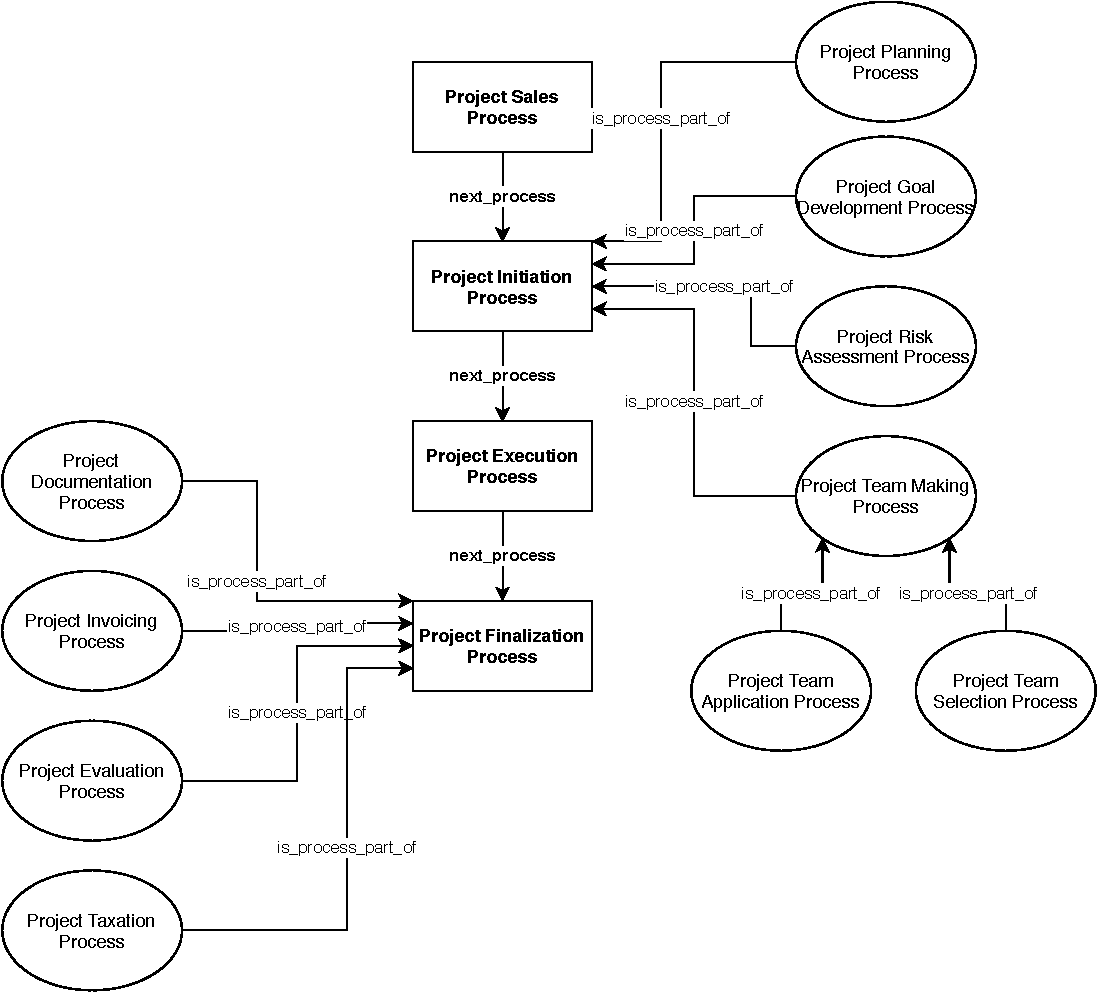
\includegraphics[width=1\textwidth]{Diagrams/project-process.pdf}
\end{figure}

\begin{figure}[h]
	\caption{Human Resources Process}
	\centering
	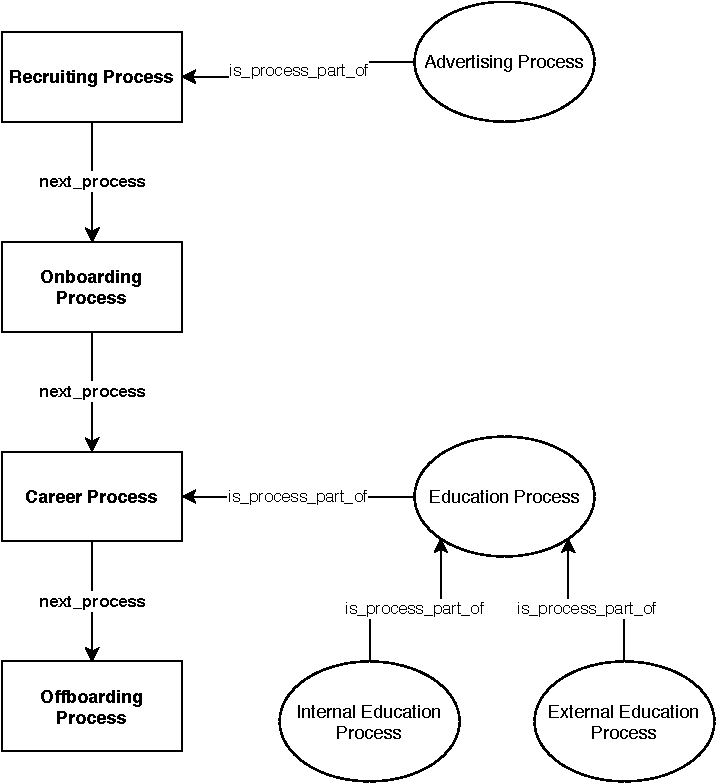
\includegraphics[width=1\textwidth]{Diagrams/hr-process.pdf}
\end{figure}

\clearpage
\printnoidxglossaries

\printbibliography

\newpage

\section{Dictionary Definitions}
\label{dictionary}
% \textcolor{gray}{\textit{\enquote{}}}

\begin{mdframed}[%
	linewidth=1pt,%
	frametitlerule=true,%
	frametitlebackgroundcolor=gray!20,%
	innertopmargin=\topskip,%
	frametitlefont=\normalfont,%
	frametitle={{\textbf{domain}} {\scriptsize\textsc{noun \hfill Merriam-Webster}}}%
	]
	
	{\small do·​main
			\begin{compactenum}
				\item law
				\begin{compactenum}
					\item complete and absolute (see absolute sense 3) ownership of land \\
					\textcolor{gray}{\enquote{\textit{our highways and roads have been in the domain of state and local governments— T. H. White b. 1915}}} \\
					 — compare eminent domain
					\item land so owned
				\end{compactenum}
				\item a territory over which dominion (see dominion sense 2) is exercised \\
				\textcolor{gray}{\enquote{\textit{The forest is part of the king's domain.}}}
				\item a region distinctively marked by some physical feature \\
				\textcolor{gray}{\enquote{\textit{a domain of rushing streams, tall trees, and lakes}}}
				\item a sphere (see sphere sense 4b) of knowledge, influence, or activity \\
				\textcolor{gray}{\textit{\enquote{the domain of biblical scholarship}, \enquote{outside the domain of city police}}}
				\item mathematics : the set of elements (see element sense 2b(3)) to which a mathematical or logical variable is limited \\
				specifically : the set on which a function (see function entry 1 sense 5a) is defined
				\item physics : any of the small randomly oriented regions of uniform magnetization in a ferromagnetic substance
				\item mathematics : integral domain
				\item biology : the highest taxonomic category in biological classification ranking above the kingdom (see kingdom sense 4b)
				\item biochemistry : any of the three-dimensional subunits of a protein that are formed by the folding of its linear peptide chain and that together make up its tertiary (see tertiary entry 1 sense 3c) structure
				\item computers : a subdivision of the Internet consisting of computers or sites usually with a common purpose (such as providing commercial information) and denoted in Internet addresses by a unique abbreviation (such as com for commercial sites or gov for government sites) \\
				\textcolor{gray}{\textit{\enquote{The domain ca is used for sites located in Canada.}}} \\
				also : domain name \\
				\textcolor{gray}{\textit{\enquote{Our domain is Merriam-Webster.com.}}}
		\end{compactenum}
	}
\end{mdframed}

\begin{mdframed}[%
	linewidth=1pt,%
	frametitlerule=true,%
	frametitlebackgroundcolor=gray!20,%
	innertopmargin=\topskip,%
	frametitlefont=\normalfont,%
	frametitle={{\textbf{vocabulary}} {\scriptsize\textsc{noun \hfill Merriam-Webster}}}%
	]
	
	{\small vo·​cab·​u·​lary \textit{\textcolor{teal}{plural}} vocabularies
		\begin{compactenum}
			\item a list or collection of words or of words and phrases usually alphabetically arranged and explained or defined : LEXICON \\
			\textcolor{gray}{\enquote{\textit{The vocabulary for the week is posted online every Monday.}}}
			\item
			\begin{compactenum}
				\item a sum or stock of words employed by a language, group, individual, or work or in a field of knowledge \\
				\textcolor{gray}{\textit{\enquote{a child with a large vocabulary}}, \enquote{the vocabulary of physicians}, \enquote{a writer known for employing a rich vocabulary}}
				\item a list or collection of terms or codes available for use (as in an indexing system) \\
				\textcolor{gray}{\enquote{\textit{… the oldest Sumerian cuneiform writing could not render normal prose but was a mere telegraphic shorthand, whose vocabulary was restricted to names, numerals, units of measure, words for objects counted, and a few adjectives.}} --- \textsc{Jared Diamon}}
			\end{compactenum}
			\item a supply of expressive techniques or devices (as of an art form) \\
			\textcolor{gray}{\textit{\enquote{an impressive musical vocabulary}}}
		\end{compactenum}
	}
\end{mdframed}

\newpage
\section{Ontology Import Links}
This work lists different ontologies in the related work section. To import them into the Protégé editor, the following links can be used:

\begin{asparadesc}
	\item [\gls{bfo}:] \url{http://purl.obolibrary.org/obo/bfo/2.0/bfo.owl}
	\item [\gls{bpmn}:] \url{https://dkm-static.fbk.eu/resources/ontologies/BPMN/BPMN_2.0_ontology.owl}
	\item [\gls{doap}:] \url{http://usefulinc.com/ns/doap}
	\item [\gls{fibo}:] \url{https://spec.edmcouncil.org/fibo/ontology/master/2019Q4.1/LoadFIBOProd.rdf}
	\item [\gls{foaf}:] \url{http://xmlns.com/foaf/spec/index.rdf}
	\item [\gls{gfo}:] \url{http://www.onto-med.de/ontologies/gfo-basic.owl}
	\item [\gls{gist}:] \url{https://ontologies.semanticarts.com/o/gistCore9.0.0.owl}
	\item [\gls{schema}:] \url{http://schema.org/version/latest/schema.rdf}
\end{asparadesc}

\section{Acknowledgments \progressbar[filledcolor=green]{1}}
This work was conducted using the Protégé resource, which is supported by grant GM10331601 from the National Institute of General Medical Sciences of the United States National Institutes of Health.

\end{document}
